\documentclass[10pt,titlepage]{article}

\usepackage{mwe}
\usepackage[hidelinks]{hyperref}

\usepackage{stz}

\tcbuselibrary{listings}

\title{\texttt{stz}}
\author{Adam Christiansen}
\date{\today}

% How to render the name of a LaTeX package.
\newcommand*{\packagename}[1]{\texttt{#1}}

% How to render inline code.
\newcommand*{\code}[1]{\texttt{#1}}

% Show LaTeX code and its result side by side.
\NewTCBListing{example}{ !O{} }{%
  % Spacing.
  boxsep=0pt,
  left=0pt,
  right=0pt,
  % Frame.
  enhanced,
  frame hidden,
  boxrule=0pt,
  lower separated=false,
  sharp corners,
  % Color.
  colback=white,
  % Layout.
  listing side text,
  halign upper=justify,
  halign lower=justify,
  % Extras.
  #1
}

\begin{document}

\maketitle
\tableofcontents
\clearpage

%==============================================================================
% Purpose
%==============================================================================

\section{Purpose}

I found myself often rewriting the same macros and configurations
over and over again every time I create a new document.
This package is my consolidated set of utilities
and opinionated set of styles and tweaks.
This document serves as a limited showcase
and set of quick visual test cases for the \code{stz} package;
This document does not give examples of every feature,
and \code{stz.sty} should be read for the full list of features.

\begin{caution}
  This package is not stable and can change at any time.
\end{caution}

%%%%%%%%%%%%%%%%%%%%%%%%%%%%%%%%%%%%%%%%%%%%%%%%%%%%%%%%%%%%%%%%%%%%%%%%%%%%%%%
%%%  _______                 _
%%% |__   __|               | |
%%%    | |_      _____  __ _| | _____
%%%    | \ \ /\ / / _ \/ _` | |/ / __|
%%%    | |\ V  V /  __/ (_| |   <\__ \
%%%    |_| \_/\_/ \___|\__,_|_|\_\___/
%%%
%%%%%%%%%%%%%%%%%%%%%%%%%%%%%%%%%%%%%%%%%%%%%%%%%%%%%%%%%%%%%%%%%%%%%%%%%%%%%%%

\section{Tweaks}

Tweaks are adjustments to LaTeX itself or external packages.

%==============================================================================
% Captions
%==============================================================================

\subsection{Captions}

Captions have \verb|\small| font sizing.

%==============================================================================
% Floats
%==============================================================================

\subsection{Floats}

The \code{table} and \code{figure} environments are adjusted to use
\code{t!} positioning and \code{\string\centering} by default.

%==============================================================================
% xcolor
%==============================================================================

\subsection{\packagename{xcolor}}

The 19 standard colors provided by \packagename{xcolor} are redefined and are
the only colors used throughout this package.

\newcommand*{\swatch}[1]{\tikz{
  \draw[draw=#1!75!black,fill=#1,thick]
    (-0.75\baselineskip,-0.5\baselineskip) rectangle (0.75\baselineskip,0.5\baselineskip);
  \node[anchor=west] at (0.75\baselineskip,0) {\texttt{\strut#1}};
}}

\noindent
\begin{tabularx}{\textwidth}{@{}XXX@{}}
  \swatch{black}     & \swatch{red}    & \swatch{blue}    \\
  \swatch{darkgray}  & \swatch{orange} & \swatch{violet}  \\
  \swatch{gray}      & \swatch{yellow} & \swatch{purple}  \\
  \swatch{lightgray} & \swatch{lime}   & \swatch{magenta} \\
  \swatch{white}     & \swatch{green}  & \swatch{pink}    \\
  {}                 & \swatch{teal}   & \swatch{brown}   \\
  {}                 & \swatch{cyan}   & \swatch{olive}   \\
\end{tabularx}

%==============================================================================
% siunitx
%==============================================================================

\subsection{\packagename{siunitx}}

These are tweaks to the \packagename{siunitx} package.

\begin{example}
% Lists, products, and ranges use a single unit and an Oxford comma.
\qtylist{1;2;5;10}{\mm}
\end{example}

\begin{example}
% Math mode is allowed in numbers.
\qty{\sim100}{\nano\volt}
\end{example}

\begin{example}
% Uncertainty is compact.
\qty{12345(67)}{\micro\ampere}
\end{example}

\begin{example}
% Powers are used when there is more than one denominator.
\qty{1}{\metre\per\second} \\
\qty{1}{\watt\per\metre\per\kelvin}
\end{example}

\begin{example}
% Several qualifiers are provided.
\qty{1}{\volt\rms}
\end{example}

%==============================================================================
% tabularx
%==============================================================================

\subsection{\packagename{tabularx}}

These are tweaks to the \packagename{tabularx} package.
The main changes are the addition of \code{L}, \code{C}, and \code{R} column types
which correspond to the \packagename{tabularx} \code{X} column
but with explicit left, centre, and right alignment.

\begin{example}
% Column alignment.
\begin{tabularx}{\linewidth}{|L|C|R|}
  \toprule
  a & b & c \\
  \midrule
  d & e & f \\
  g & h & i \\
  \bottomrule
\end{tabularx}
\end{example}

The column width can be adjusted by changing the column width weight.
It is important that the weights sum up to the number of columns.
This can also change the behviour of cells spanning multiple columns.

\begin{example}
% Column size.
\begin{tabularx}{\linewidth}{ |>{\colww{0.5}}L |>{\colww{1.5}}C|R|}
  \toprule
  0.5 & 1.5 & 1.0 \\
  \midrule
  d & e & f \\
  g & h & i \\
  \bottomrule
\end{tabularx}
\end{example}

%==============================================================================
% TikZ and PGF
%==============================================================================

\subsection{Ti\textit{k}Z and PGF}

Several defaults are changed for \packagename{tikz} and \packagename{pgf}.
The most apparent are plots.

{
\pgfplotsset{height=1.25\linewidth}
\begin{example}
\pgfplotsset{domain=0:1,samples=6}
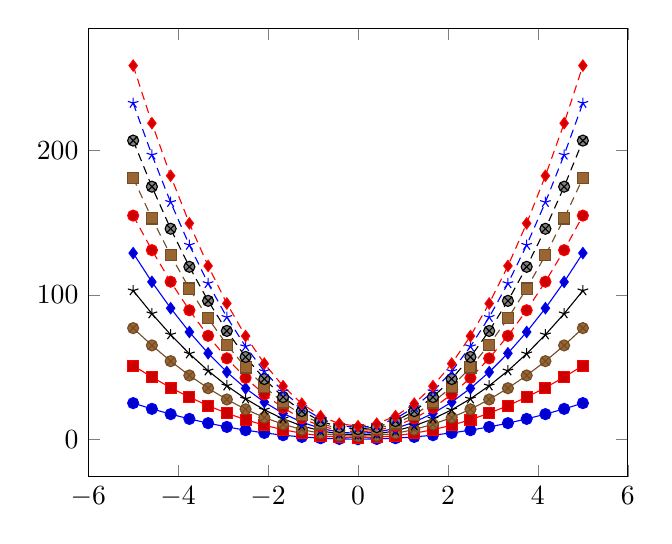
\begin{tikzpicture}
  \begin{axis}
    \addplot+ { 1*x^2+0};
    \addplot+ { 2*x^2+1};
    \addplot+ { 3*x^2+2};
    \addplot+ { 4*x^2+3};
    \addplot+ { 5*x^2+4};
    \addplot+ { 6*x^2+5};
    \addplot+ { 7*x^2+6};
    \addplot+ { 8*x^2+7};
    \addplot+ { 9*x^2+8};
    \addplot+ {10*x^2+9};
  \end{axis}
\end{tikzpicture}
\end{example}
}

%%%%%%%%%%%%%%%%%%%%%%%%%%%%%%%%%%%%%%%%%%%%%%%%%%%%%%%%%%%%%%%%%%%%%%%%%%%%%%%
%%%  ______ _                           _
%%% |  ____| |                         | |
%%% | |__  | | ___ _ __ ___   ___ _ __ | |_ ___
%%% |  __| | |/ _ \ '_ ` _ \ / _ \ '_ \| __/ __|
%%% | |____| |  __/ | | | | |  __/ | | | |_\__ \
%%% |______|_|\___|_| |_| |_|\___|_| |_|\__|___/
%%%
%%%%%%%%%%%%%%%%%%%%%%%%%%%%%%%%%%%%%%%%%%%%%%%%%%%%%%%%%%%%%%%%%%%%%%%%%%%%%%%

\section{Elements}

Elements are new features.

%==============================================================================
% Admonitions
%==============================================================================

\subsection{Admonitions}

Admonitions provide highlighted notes with context.

\begin{example}
\begin{note}
  A note that stands out.
\end{note}
\end{example}

\begin{example}
\begin{tip}
  Optional tip.
\end{tip}
\end{example}

\begin{example}
\begin{important}
  Important information.
\end{important}
\end{example}

\begin{example}
\begin{caution}
  Potential risk.
\end{caution}
\end{example}

\begin{example}
\begin{danger}
  Negative consequences.
\end{danger}
\end{example}

Admonitions can also appear inline.

\begin{example}
\tipinline{message} \\
\noteinline{message} \\
\importantinline{message} \\
\cautioninline{message} \\
\dangerinline{message}
\end{example}

%==============================================================================
% Todo
%==============================================================================

\subsection{Todo}

% Todo notes emit warnings. The uses of todo in this section are intended and
% the warnings will not be legitimate, so warnings are temporarily disabled
% then enabled again at the end of the section.
\makeatletter
\let\old@stz@warning\@stz@warning
\let\@stz@warning\@gobble
\makeatother

Add todo notes to indicate work that must still be done.
All todo notes emit warnings in the log.

\begin{example}
\begin{todo}
  A big note.
\end{todo}
\end{example}

\begin{example}
Highlight \todoadd{text} to add.
\todoadd{}
\end{example}

\begin{example}
Highlight \todoremove{text} to remove.
\todoremove{}
\end{example}

\begin{example}
Highlight \todofix{text} to fix.
\todofix{}
\end{example}

\begin{example}
Highlight \todorevise{text} to revise.
\todorevise{}
\end{example}

\begin{example}
A \todocite{citation} is required.
\todocite{}
\end{example}

\begin{example}
Cross \todoref{reference} required.
\todoref{}
\end{example}

\begin{example}
More \todomore{text} required.
\todomore{}
\end{example}

\begin{example}
% Can include optional number of sentences.
\todosentence
% \todosentence[2] % 2 sentences.
\end{example}

\begin{example}
% Can include optional number of paragraphs.
\todopar
% \todopar[2] % 2 paragraphs
\end{example}

{
\stzsetup{todo/box/.cd,height=2.5cm,width=\linewidth}
\begin{example}
% Useful for placeholder figures and tables.
\todobox
\end{example}
}

% Enable warnings again.
\makeatletter
\let\@stz@warning\old@stz@warning
\let\old@stz@warning\undefined
\makeatother

%==============================================================================
% Annotations
%==============================================================================

\subsection{Annotations}

Annotations are used to draw on top of graphics.

\begin{example}
\begin{annotatedgraphic}%
    [width=0.8\linewidth]%
    {example-image}
  \node at (0.4, 0.7) {$\pi$};
\end{annotatedgraphic}
\end{example}

A help grid can be added to assist in label positioning.

\begin{example}
\begin{annotatedgraphic}%
    [width=0.8\linewidth]%
    {example-image}
  \annotationhelplines
  \node at (0.4, 0.7) {$\pi$};
\end{annotatedgraphic}
\end{example}

\end{document}
